\documentclass[12 pt]{article}
\usepackage{fancyhdr}
\usepackage[margin = 1 in]{geometry}
\usepackage{amsmath}
\usepackage{enumerate}
% \usepackage{indentfirst}
\pagestyle{fancy}
\usepackage{graphicx}
\usepackage[version=3]{mhchem}
\fancyhf{}
\usepackage{sectsty}	
\lhead{Andrew Wang}
\chead{CS/CNS/EE 155 Machine Learning \& Data Mining}
\rhead{Yue}
\sectionfont{\fontsize{15}{18}\selectfont}
\usepackage{graphicx}
\usepackage{array}
\newcolumntype{P}[1]{>{\centering\arraybackslash}p{#1}}
\newcolumntype{M}[1]{>{\centering\arraybackslash}m{#1}}
\usepackage[font=small,labelfont=bf]{caption}
\usepackage{float}
\usepackage{float}
\usepackage{subfig}
\usepackage{microtype}
\usepackage{ amssymb }
\usepackage{amsmath}
\usepackage{commath}
\usepackage{bbm}

\begin{document}
	\begin{center}
		\section*{Homework 3}
	\end{center}
	
	
	\subsection*{1 Decision Trees}	
	\noindent\textbf{Question A:}  \\
	\noindent \textbf{i. Entropy}: For the root node, p$_{s'}$ = 0.75 and - $\abs{S'}$ = 4, so our entropy is 3.2451124978365313. \\ \\
	For the first level: 
	\begin{itemize}
		\item Package type: Bagged = $\{$yes, yes$\}$, Canned = $\{$yes, no$\}$ so entropy is 2.0.
		\item Unit price $>$ $\$$5: Yes = $\{$no, yes$\}$, No = $\{$yes, yes$\}$ so entropy is 2.0.
		\item Contains $>$ 5 grams of fat: Yes = $\{$no, yes$\}$, No = $\{$yes, yes$\}$ so entropy is 2.0
	\end{itemize}
	Because all have the same entropies, we arbitrarily choose to split on unit price.  \\ \\
	
	For the second level: 
	\begin{itemize}
		\item Package type: Bagged = $\{$yes$\}$, Canned = $\{$no$\}$ so entropy is 1.0.
		\item Contains $>$ 5 grams of fat: Yes = $\{$no$\}$, No = $\{$yes$\}$ so entropy is 1.0.
	\end{itemize}
	Both have the same entropy, so we arbitrarily choose to split on package type. Now, we have no more impurities and are done. For impurity calculations, we subtract entropies of consecutive levels. From root to level 1, we had an impurity reduction of 3.245 - 2.0 = 1.245 and from level 1 to level 2, we had an impurity reduction of 2.0 - 0.0 = 2.0. 
	
	\begin{figure}[H]
	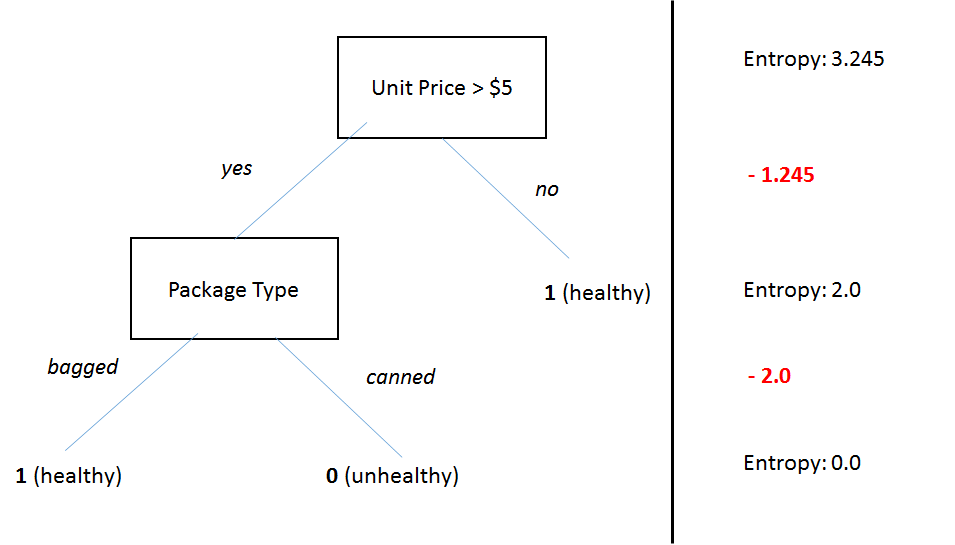
\includegraphics[width=17cm]{tree1}
	\end{figure}
	
	
	\noindent\textbf{ii. Gini index}:  For the root node, p$_{s'}$ = 0.75 and - $\abs{S'}$ = 4, so our entropy is 1.5. \\ \\
	For the first level: 
	\begin{itemize}
		\item Package type: Bagged = $\{$yes, yes$\}$, Canned = $\{$yes, no$\}$ so entropy is 1.0.
		\item Unit price $>$ $\$$5: Yes = $\{$no, yes$\}$, No = $\{$yes, yes$\}$ so entropy is 1.0.
		\item Contains $>$ 5 grams of fat: Yes = $\{$no, yes$\}$, No = $\{$yes, yes$\}$ so entropy is 1.0
	\end{itemize}
	Because all have the same entropies, we arbitrarily choose to split on unit price.  \\ \\
	
	For the second level: 
	\begin{itemize}
		\item Package type: Bagged = $\{$yes$\}$, Canned = $\{$no$\}$ so entropy is 1.0.
		\item Contains $>$ 5 grams of fat: Yes = $\{$no$\}$, No = $\{$yes$\}$ so entropy is 1.0.
	\end{itemize}
	Both have the same entropy, so we arbitrarily choose to split on package type. Now, we have no more impurities and are done. For impurity calculations, we subtract entropies of consecutive levels. From root to level 1, we had an impurity reduction of 1.5 - 1.0 = 0.5 and from level 1 to level 2, we had an impurity reduction of 1.0 - 0.0 = 1.0. 
	
	\begin{figure}[H]
		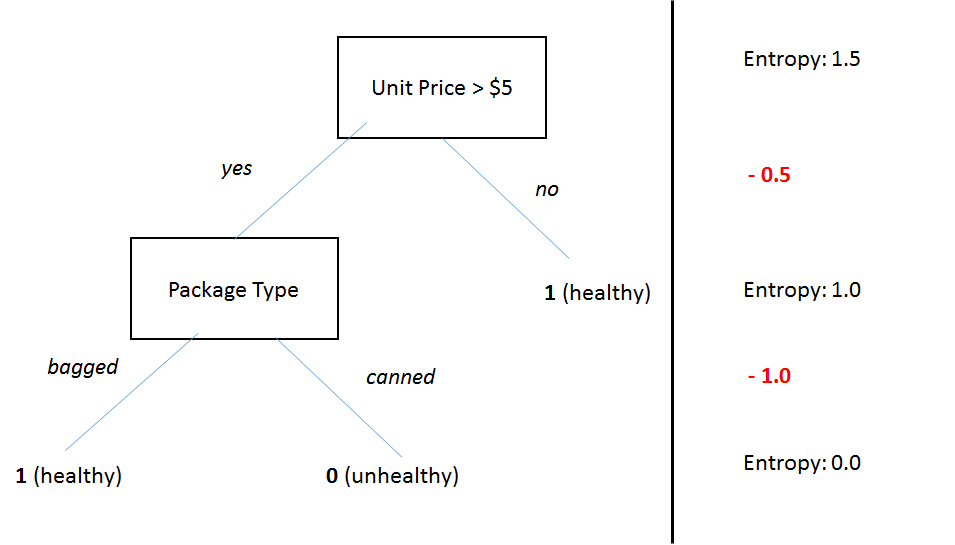
\includegraphics[width=17cm]{tree2}
	\end{figure}
	\noindent\textbf{Question B:} No, a decision tree is NOT always preferred for classification problems in comparison to a linear classifier. We can see that in the example below where linear SVM can easily find max margin but decision trees require complex axis-aligned partitioning.  \\
	\begin{figure}[H]
	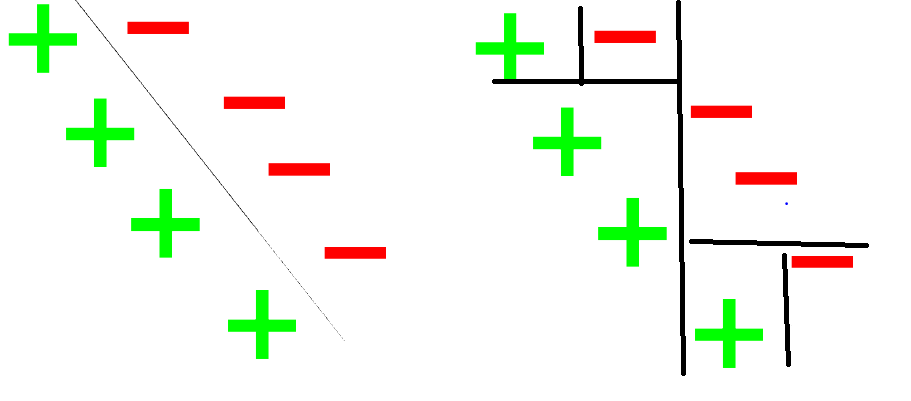
\includegraphics[width=17cm]{treesvm}
	\end{figure}	
	\noindent\textbf{Question C:}  \\\textbf{i.} No matter how we split the data, the entropy will remain at 2.0. Thus, we do not split at all. The classification error is 1/2 = 0.5. The resulting tree is a single root node, corresponding to entire data set and makes a single prediction based on majority class in set. \\
	\begin{figure}[H]
		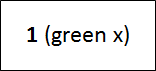
\includegraphics[width=5cm]{smallTree}
	\end{figure}	
	\noindent \textbf{ii.} Given that x$_1$ is the horizontal axis and x$_2$ is the vertical axis, a two-level decision tree that classifies the above dataset with zero classification error is as follows:
	\begin{figure}[H]
	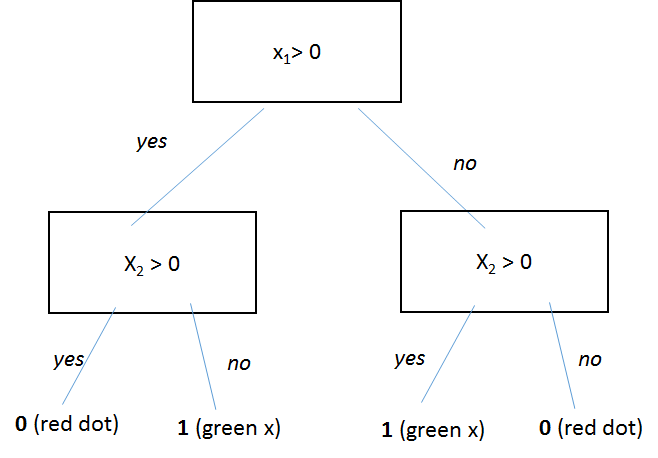
\includegraphics[width=12cm]{validTree}
	\end{figure}	
	
	\noindent To classify this case, we use the impurity measure of: \\
	L(S') = $\frac{\text{\# pos * \# neg}}{\sqrt{\text{S'}}}$ \\ \\
	\noindent Pros: This would guarantee that if the percentage of correct classifications before the split is equal to the percentage of correct classifications after a split (like the example above), we would go ahead and split (as the sqrt term in the denominator ensures impurity after such a split would be less).  \\
	
	\noindent Cons: Because this encourages splitting when other impurity measures may not, this may be prone to overfitting. Sometimes we may not want to split in a situation where percentage of correct classification remains steady to improve generalization.  \\ 
	
	
	\noindent \textbf{iii.} The largest number of unique thresholds one needs in order to achieve zero classification error in a dataset of one hundred points is 99. In general, the number of unique splits is (n-1) where n is the size of the dataset. We can see this by looking at datasets of smaller size. For 3 points, we can easily see that it only requires two splits, for 4 points, we require three splits, and for 5 points, we require four splits. We can easily see that by adding a new point, we only require one more split to isolate the new point from the previous points. Thus, every time we add 1 point, we need 1 more split for perfect classification. Thus, when we have 100 points, we only need 99 splits. \\

	\noindent\textbf{Question D:} From the lecture slides, we know that number of possible queries is equal to the number of splits = D * N. Thus, our worst-case complexity is O(N * D). \\
	
 
	
	\subsection*{2 Overfitting Decision Trees}
	\noindent\textbf{Question A:} 
	\begin{figure}[H]
		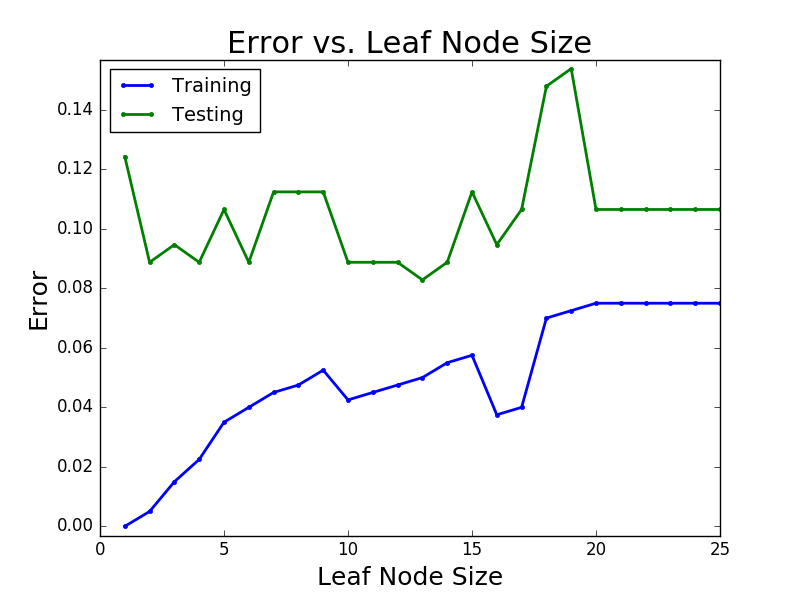
\includegraphics[width=13cm]{leafNode}
	\end{figure}	
	
	\noindent\textbf{Question B:} 
	\begin{figure}[H]
		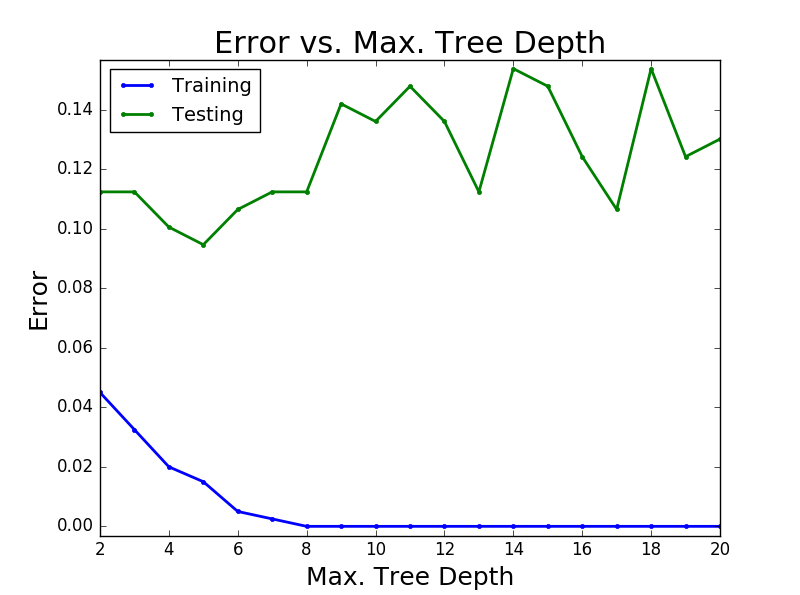
\includegraphics[width=13cm]{maxTreeDepth}
	\end{figure}	

	%\begin{figure}[h]
	%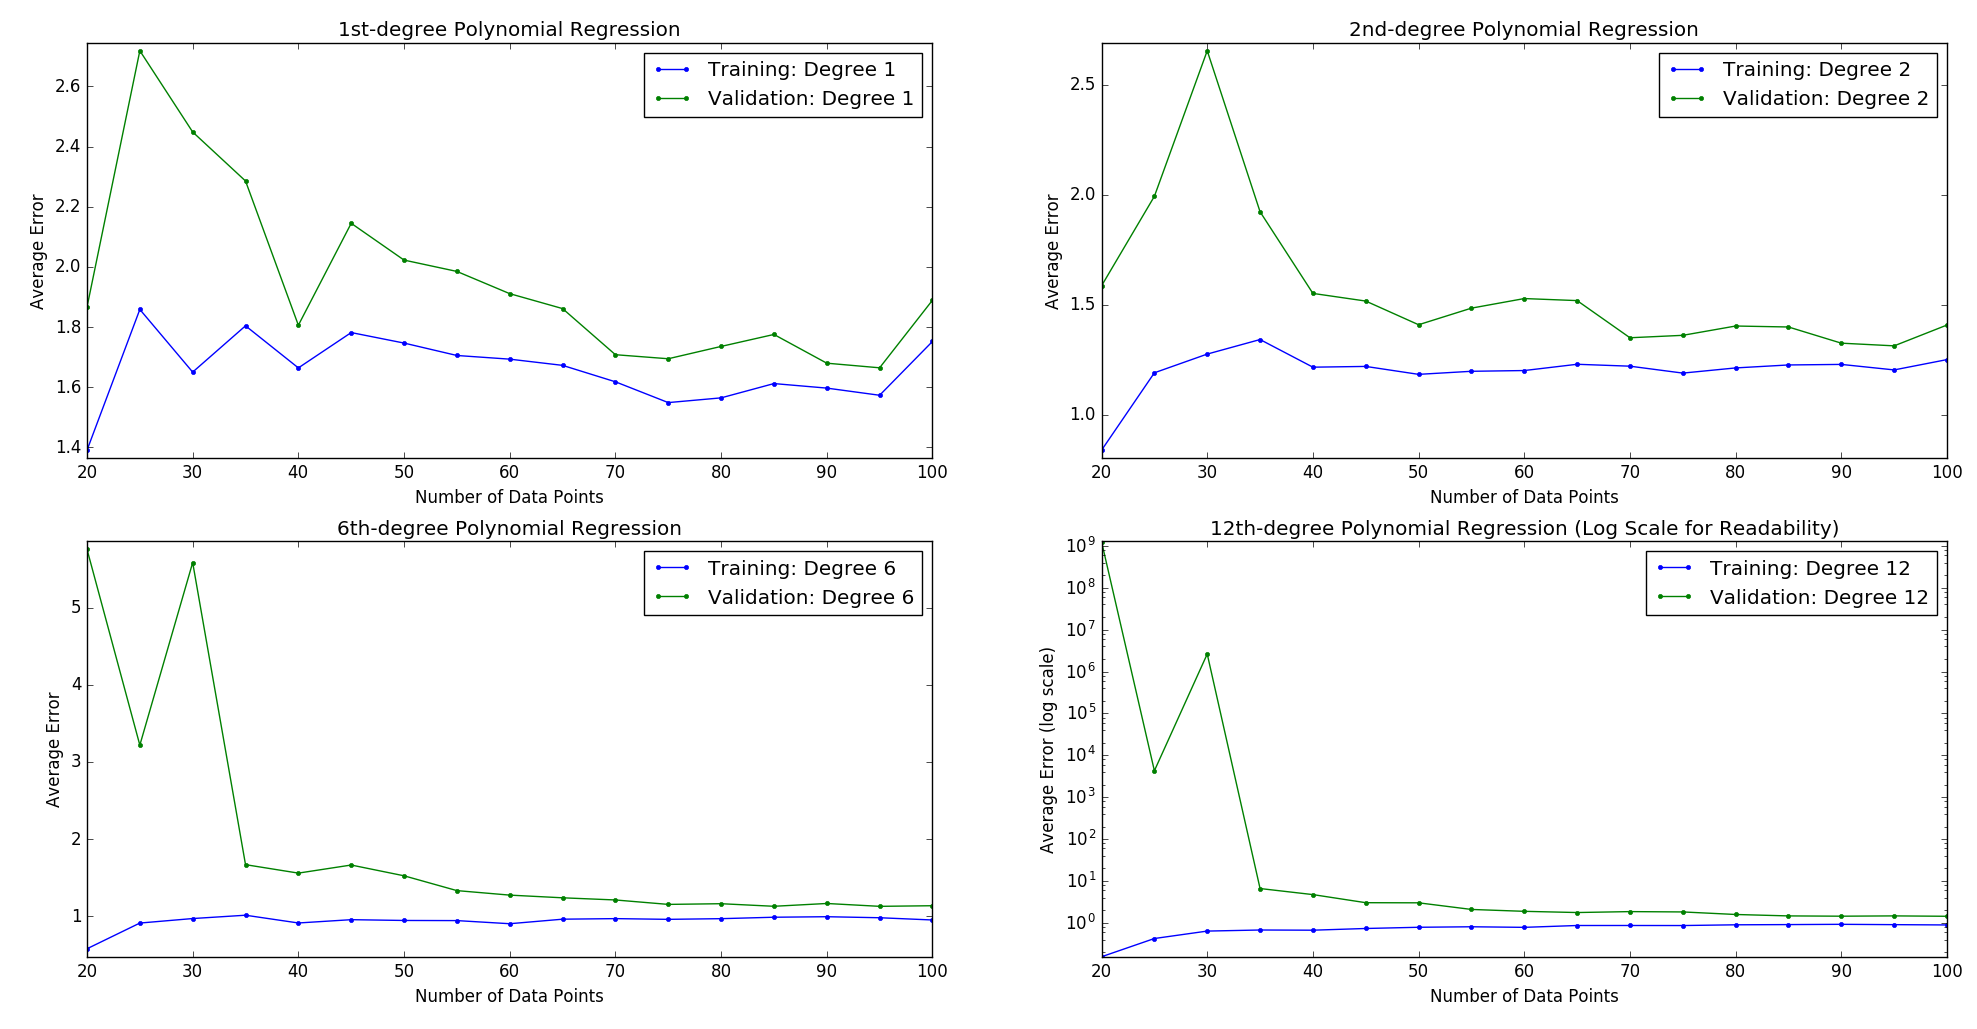
\includegraphics[width=17cm]{LearningCurves}
	%\end{figure}	
	
	\noindent\textbf{Question C:}  \\
	\noindent For the plot of "Error vs. Leaf Node Size," early stopping occurs as leaf node size increases (meaning less splits).  Without early stopping such as when leaf node size is 1, we have overfitting (low training error, but high testing error). However, as we increase the leaf node size and introduce stopping, the testing error decreases, suggesting better generalization. It is also important to note that when there is too much early stopping, the testing error can shoot up (when min. leaf node size is between 16 and 20) suggesting underfitting. Thus, early stopping helps prevent overfitting and improves generalization, but we must also make sure we do not stop too early. \\
	
	\noindent For the plot of "Error vs. Max. Tree Depth," early stopping occurs as max. tree depth decreases (meaning less splits).  Without early stopping such as when the max. tree depth is large, we have overfitting (low training error, but high testing error). However, as we decrease the max. tree depth (less than 10), the testing error decreases, suggesting better generalization. It is also important to note that when there is too much early stopping, the testing error can shoot increase (when max. tree depth is less than 6) suggesting underfitting. Thus, once again, early stopping helps prevent overfitting and improves generalization, but we must also make sure we do not stop too early. \\
	
	\subsection*{3 The AdaBoost Algorithm}
	\noindent\textbf{Question A:} \\
	To show:
	\[ E = \frac{1}{N} \sum_{i = 1}^N \exp(-y_i f(x_i)) \geq \frac{1}{N} \sum_{i = 1}^N
	\mathbbm{1} (H(x_i) \neq y_i) \]
	
	we only need to show that for $x_i, y_i$,
	
	\[ \exp(-y_i f(x_i)) \geq \mathbbm{1} (H(x_i) \neq y_i) \]
	

	If $y_i$ and $f(x_i)$ are opposite signs, 
	\[ \exp(-y_i f(x_i)) = \exp(\textit{nonnegative number}) \geq 1 \]
	\[ \mathbbm{1} (H(x_i) \neq y_i) = 1 \]
	
	Thus, \[ \exp(-y_i f(x_i)) \geq \mathbbm{1} (H(x_i) \neq y_i) \]
	
	Now, if $y_i$ and $f(x_i)$ have the same sign,
	\[ \exp(-y_i f(x_i)) = \exp(\textit{negative number}) \geq 0 \]
	\[ \mathbbm{1} (H(x_i) \neq y_i) = 0 \]

	Thus, 
	\[ \exp(-y_i f(x_i)) \geq \mathbbm{1} (H(x_i) \neq y_i) \]
	
	Then combining the two above scenarios:
	\[ \exp(-y_i f(x_i)) \geq \mathbbm{1} (H(x_i) \neq y_i) \]
	
	Thus we have shown that
	\[ E = \frac{1}{N} \sum_{i = 1}^N \exp(-y_i f(x_i)) \geq \frac{1}{N} \sum_{i = 1}^N
	\mathbbm{1} (H(x_i) \neq y_i) \]
	
	\noindent\textbf{Question B:} \\
	We start with a formula provided from lecture:
	\[ D_{t+1}(i) = \frac{D_t(i) \exp(-\alpha_t y_i h_t(x_i))}{Z_t} \]
	
	Now, from this, we express $D_t(i)$:
	
	\[ D_t(i) = D_1(i) \cdot\Big(  \prod_{j = 1}^{t - 1} \frac{\exp(-\alpha_j y_i h_j(x_i))}{Z_j} \Big)\]
	
	Then, plugging $D_t(i)$ into the $Z_t$ formula from the problem, we get:
	
	\[ Z_T = \sum_{i = 1}^T \Big( \prod_{j = 1}^{T - 1} \frac{\exp(-\alpha_j y_i h_j(x_i))}{Z_j} \Big)
	\cdot D_1(i) \cdot \exp(-\alpha_T y_i h_T(x_i)) \]
	
	\[ Z_T = \sum_{i = 1}^T \Big( \prod_{j = 1}^{T - 1} \frac{1}{Z_j} \Big) \cdot
	\Big( \prod_{j = 1}^{T - 1} \exp(-\alpha_j y_i h_j(x_i)) \Big)
	\cdot D_1(i) \cdot \exp(-\alpha_T y_i h_T(x_i)) \]
	
	\[ Z_T = \sum_{i = 1}^T \Big( \prod_{j = 1}^{T - 1} \frac{1}{Z_j} \Big) \cdot
	\Big( \prod_{j = 1}^{T} \exp(-\alpha_j y_i h_j(x_i)) \Big)
	\cdot D_1(i) \]
	
	We know that $\Big( \prod_{j = 1}^{T} \exp(-\alpha_j y_i h_j(x_i)) \Big) = \exp(-y_i \sum_{j = 1}^T \alpha_j h_j(x_i)$, so we can substitute: 
	
	
	\[ Z_T = \sum_{i = 1}^T \Big( \prod_{j = 1}^{T - 1} \frac{1}{Z_j} \Big) \cdot
	\exp(-y_i \sum_{j = 1}^T \alpha_j h_j(x_i))
	\cdot D_1(i) \]
	
	\[ Z_t = \sum_{i = 1}^T \Big( \prod_{j = 1}^{T - 1} \frac{1}{Z_j} \Big) \cdot
	\exp(-y_i f(x_i))
	\cdot D_1(i) \]
	
	\[ \Big( \prod_{j = 1}^{T - 1} Z_j \Big) \cdot Z_T = \sum_{i = 1}^T
	\exp(-y_i f(x_i))
	\cdot D_1(i) \]
	
	\[ \prod_{j = 1}^{T} Z_j = \sum_{i = 1}^T \exp(-y_i f(x_i)) \cdot D_1(i) \]
	
	Finally, setting $D_1(i) = \frac{1}{T}$ to
	get:
	
	\[ E = \frac{\sum_{i = 1}^T \exp(-y_i f(x_i))} {T}\]
	
	
	
	
	\noindent\textbf{Question C:} 
	\noindent We first seek to show that 
	\[Z_t = (1 -\epsilon_t)\exp(-\alpha_t) + \epsilon_t \exp(\alpha_t)\] 
	
	We break this problem down into two cases:
	
	When h$_{t}(x_i) \neq y_i$:
	
	Using the formula from part B: 	\[ Z_t = \sum_{i = 1}^T \Big( D_t(i)\exp(-\alpha_t y_i h_t (x_i))\Big) \]
	
	\[ Z_t = \sum_{i = 1}^T \Big( D_t(i)\exp(\alpha_t)\Big) \]
	\[ Z_t = \Big(\exp(\alpha_t)\Big) \]
	
	Using the formula we are trying to show:
	
	We first know that $\epsilon_t$ = $\sum_{i=1} ^ N (D_t(i)$ $\mathbbm{1}$ $(h_t(x_i) \neq y_i)$. In this case where  $(h_t(x_i) \neq y_i)$, $\epsilon_t$ = 1, and thus:
	
	\[Z_t = (1 -\epsilon_t)\exp(-\alpha_t) + \epsilon_t \exp(\alpha_t)\] 
		
	\[Z_t = (0)\exp(-\alpha_t) + 1 \exp(\alpha_t)\] 
	\[Z_t = \exp(\alpha_t)\] which matches the formula from part B.\\
	
	Now, the second case, when h$_{t}(x_i) = y_i$:
	
	Using the formula from part B: 	\[ Z_t = \sum_{i = 1}^T \Big( D_t(i)\exp(-\alpha_t y_i h_t (x_i))\Big) \]
		
		\[ Z_t = \sum_{i = 1}^T \Big( D_t(i)\exp(-\alpha_t)\Big) \]
		\[ Z_t = \Big(\exp(-\alpha_t)\Big) \]
		\[ Z_t = \Big(\exp(-\alpha_t)\Big) \]
		
	Using the formula we are trying to show: 
	In this case, $\epsilon_t$ = 0, so 
		\[Z_t = (1 -\epsilon_t)\exp(-\alpha_t) + \epsilon_t \exp(\alpha_t)\] 
	
	\[Z_t = (1)\exp(-\alpha_t) + 0 \exp(\alpha_t)\] 
	\[Z_t = \exp(-\alpha_t)\] which matches the formula from part B.\\
	
	Thus, we have shown that the normalizer Z$_t$ can be written as 	\[Z_t = (1 -\epsilon_t)\exp(-\alpha_t) + \epsilon_t \exp(\alpha_t)\].
	
	Taking the derivative with respect to $\alpha_t$ and setting equal to zero for minimization:
	
	\[ \frac{\partial Z_t}{\partial \alpha_t} = (1 - \epsilon_t)(-\alpha_t)\exp(-\alpha_t)
	+ \epsilon_t \alpha_t \exp(\alpha_t) = 0 \]
	
	\[ \epsilon_t \alpha_t \exp(\alpha_t) = \alpha_t (1 - \epsilon_t) \exp(-\alpha_t) \]
	
	\[ \alpha_t \exp(2 \alpha_t) =\alpha_t \frac{1 - \epsilon_t}{\epsilon_t} \]
	
	\[ \exp(2 \alpha_t) = \frac{1 - \epsilon_t}{\epsilon_t} \]
	
	\[ \alpha_t = \frac{1}{2} \ln \Big(\frac{1 - \epsilon_t}{\epsilon_t} \Big) \]
	
	\[ \implies \alpha^*_t = \frac{1}{2} \ln \Big(\frac{1 - \epsilon_t}{\epsilon_t} \Big) \]
	
	
	
\end{document}